\subsection{Objects in the amber.showoff package}


\begin{figure}[htp]
  \centering
  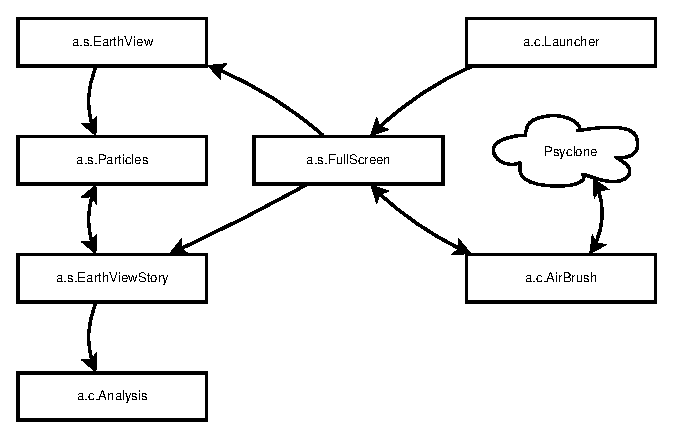
\includegraphics{image/showoff-fullscreen}
  \caption{\label{fig:showoff-fullscreen}Object model of the full screen
    ShowOff module. Arrows represent the presence of references to the object
    where it is pointing to in the object where it is pointing from. The object
    model of the applet is about equal to this one.}
\end{figure}


\classname{EarthView}

\begin{classmetadata}
  \extends{javax.swing.JPanel}
  \implements{Runnable}
  \dependencies{FullScreen, StoryLauncher}
  \function{EarthView is a graphical user interface element based on a JPanel
      which displays a picture of Earth in space, with particles orbiting
      around it. Attractors can be added to influence the orbits of the
      particles.}
  \processing{There is a list of particles, which contains information on
      their location and more. EarthView draws each of the particles in the
      list on itself.}
\end{classmetadata}

\begin{interface}
  \init{EarthView}{\mbox{Collection$\langle$Particle$\rangle$} pc}
    {Initializes the EarthView display. It is a child of JPanel and can as such
    be used inside any Swing application. Before starting the Earthview, first
    couple a Particle collection to it using setParticleCollection.}
    \method{\void}{setParticleCollection}{\mbox{Collection$\langle$Particle$\rangle$} pc}
    {Sets the collection of particles to be displayed in the view.}
  \method{\void}{run}{}
    {Runs the thread (for Runnable).}
  \method{\void}{start}{}
    {Starts the thread, lets EarthView draw stuff.}
\end{interface}



\classname{FullScreen}

\begin{classmetadata}
  \extends{amber.ShowOff}
  \implements{amber.common.AirBrushCallable}
  \dependencies{ShowOff}
  \function{This is a ShowOff module which displays the visualization in full
    screen size.}
\end{classmetadata}

\begin{interface}
  \init{FullScreen}{}
    {Initializes something.}
  \method{\void}{start}{}
    {Start the visualization.}
  \method{void}{airBrushReceiveMessage}{Message msg}
    {}
\end{interface}



\classname{Particle}

\begin{classmetadata}
  \function{Storage of particle data.}
  \data{An object of this class has information about its location and
    velocity, and it knows from which story it originates.}
  \dependencies{StoryLauncher, Particles}
\end{classmetadata}

\begin{interface}
  \init{Particle}{Story s}
    {Initializes a particle for Story s.}
  \method{\void}{launch}{}
    {Launches the particle, all parameters must be set, they cannot be changed
      afterwards.}
  \method{\void}{boost}{double}
    {Boost the particle in the direction it is heading. This can happen when
      for instance the Story gets replies or comments; boosting keeps the
      particle around longer.}
  \method{double}{getMass}{}
    {Gets the mass of the particle}
  \method{Point2d}{getLocation}{}
    {Gets the location}
  \method{Vector2d}{getVelocity}{}
    {Gets the velocity}
  \method{Vector2d}{getAcceleration}{}
    {Gets the acceleration}
  \method{\void}{calculate}{double t}
    {Calculates and sets new values using the current values after a period of
      time t}
\end{interface}

The Particles' location is represented by polar coordinates, with ``earth''
being the origin (0, 0).

A particle can be in one of five states: new, launch, orbit, boost or crashed.
Every particle will obviously start in the ``new'' state, after which it is
launched and gets into ``launch'' state. In this state, the $r$ component will
grow until it reaches a set height above the surface of earth, while $\theta$
also accellerates to a set speed. When these values are reached, the particle
will be in orbit and thus in state ``orbit''.

In orbit, a particle slows down and slowly falls back to the earth until it
reaches some lower bound when it is considered ``crashed''. While a particle is
in orbit, it can get a speed increase, it will get in ``boost'' state. During
this period, the height and speed are increased, hereby keeping the particle
orbiting earth for a prolonged time.

While in orbit, a particle can also be attracted by certain attractors that are
located outside the orbits, dependent on the topic of the story it represents.

\classname{Applet}

\begin{classmetadata}
  \extends{amber.ShowOff}
\end{classmetadata}

% \begin{interface}
% \end{interface}

